\section{Database Subsystem}
This section talks about concepts that are most relevant to a decentralized world: distributed query processing, dynamic clustering, data sovereignty and decentralized fine-grained access control. It also discusses well understood database concepts like byzantine paxos, role of timestamps in achieving external consistency, distributed transactions etc.
\subsection{Distributed query processing} High level architecture of a Picolo node looks like \figref{fig:node_arch}
\begin{figure}[h!] \centering
	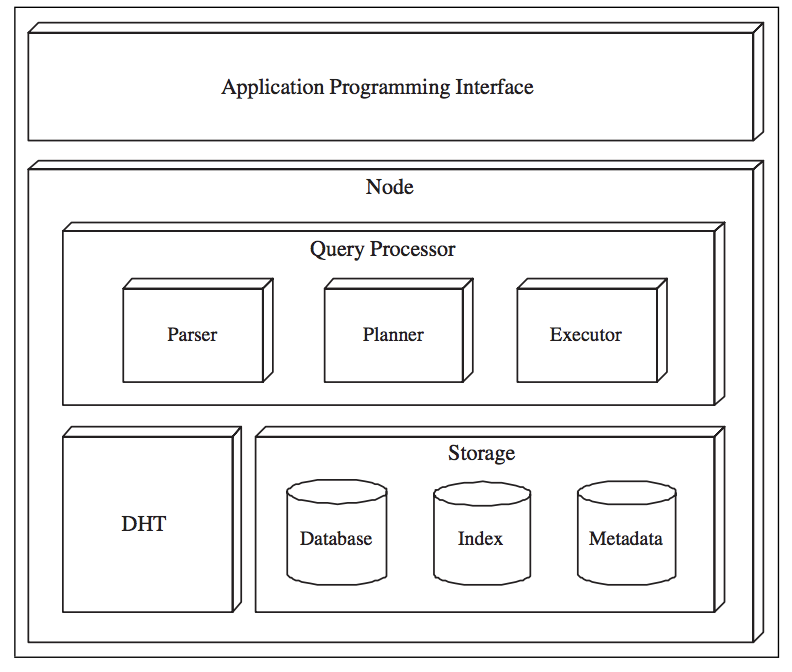
\includegraphics[width=\fscale{1}]{node_arch.png}
	\caption{A Picolo node}
	\label{fig:node_arch}
\end{figure}
The metadata depicted in the figure contains schema metadata to be exposed to the world. Nodes that wish to keep data private should not export the data's metadata to the metadata container. Suppose there is a table called \textit{users} with four columns: \textit{username}, \textit{firstname}, \textit{lastname} and \textit{email}. The exported metadata entry might look like:
\begin{center}
	\begin{tabular}{| c | c |} 
		\hline
		Entity & Keywords \\ [0.5ex] 
		\hline
		users & user, people, customer, profile\\ 
		\hline
		name & name \\
		\hline
		firstname & fn, {f\_name}, {first\_name} \\
		\hline
		lastname & ln, {l\_name}, {last\_name} \\
		\hline
		email & id, contact \\ [1ex] 
		\hline
	\end{tabular}
\end{center}
When a query is posed to any node in the system, the node first tries to fulfill it with a local query before passing it along to its neighbors. Remember, nodes in the system host data with heterogeneous schemas. Hence the keywords are used to find semantically similar data. Similarity metrics that determine whether a query matches a heterogeneous schema are not discussed here.
\subsection{Dynamic clustering} \label{sec:dynamic_cluster}
Semantic proximity metrics are used to find nodes that are hosting semantically similar schemas. Overtime, these nodes are discovered and are clustered together for better query performance by reducing the number of network hops required.
\subsection{Data sovereignty}
Picolo supports two different schema types: \textit{application controlled} and \textit{user controlled}. Applications can use user controlled schemas to put users in absolute control of data and better comply with regulations like GDPR. For example, a decentralized twitter may  want users to have control over their tweets. Users can use any third party client or Picolo's official clients to interact with their tweets effectively rendering the decentralized twitter just another client to the data albeit with better features. \newline\newline
When semantics don't allow to put user in control of data, application controlled schemas can be used. An example here would be a decentralized ticketing application where users should not be given fine grained control to selectively delete data about which tickets they bought.
\subsection{Access control} \label{sec:access_control}
Applications and users may want to share data with other parties but may wish to impose access controls. There are a few ways of achieving this including building an API on top of the data or using proxy re-encryption techniques. We use a secret sharing scheme instead as it gels well with p2p nature of the system and does not introduce asymmetry like other solutions. Rules can be defined by a SQL like declarative language at any granularity desired like at the level of a single row or a cell. An example row level granularity rule looks like:\newline \newline
\texttt{SELECT  * \newline FROM users \newline WHERE email=foo@bar.com \newline NODE (SELECT nodeId FROM nodes WHERE domain=application)} \newline \newline
An example value level (only username is given access to) granularity rule looks like:\newline \newline
\texttt{ SELECT username \newline FROM users \newline WHERE email=foo@bar.com \newline NODE (SELECT nodeId FROM nodes)}\newline\newline
Here \texttt{NODE} is a new clause we introduce to SQL dialect.
\subsection{Consensus, replication, sharding} \label{sec:paxos}
\textbf{data locality}: 
\newline\newline
\textbf{auto heal}: Cluster can fail. What happens when data poisoning happens. What if the whole replica set disappears. Make sure there are no correlated failures. Use geo ip to replicate to different regions. Cluster means a large number of nodes in the same network - think a mini datacenter. How to ensure data is closes to users and follow constraints like it doesn't leave a jurisdiction
Paxos based sync replication and consensus. Data needs to be sharded automatically. Same as cdb.
\subsection{Distributed transactions and hybrid time}
Using atomic clocks, google external ntp service, stratum 1 ntp servers. Use logical time appended to physical time. Handle clock skew. Nodes that drift too apart should die. 
\newline\newline
\textbf{mvcc}: Keys have timestamps and queries can be made in the past or fetched from a snapshot in the past. Client configurable backup and restore mechanisms. How does this affect data sovereignty?

